\section{方法}\label{sec:method}
本节先形式化观测支持（\ref{sec:3_1}），再给出 ALFNet 的整体数据流（\ref{sec:3_2}），随后按数据流依次介绍观测支持感知历史补全（SAHC，\ref{sec:3_3}）、观测条件化图预测（ALFGraph，\ref{sec:3_4}）、空间上下文时间条件分支（ALFTemporal）与 FiLM 调制（\ref{sec:3_5}）和角色缩放图修正（\ref{sec:3_6}），最后说明训练目标（\ref{sec:3_7}）与数据集特定设置（\ref{sec:3_8}）。

\subsection{问题设置与观测支持}\label{sec:3_1}

路网表示为静态图 $\mathcal{G}=(\mathcal{V},\mathbf{A})$，其中 $|\mathcal{V}|=N$，$\mathbf{A}\in\mathbb{R}^{N\times N}$ 为加权邻接矩阵；全部节点的拓扑及可用静态属性在各阶段均可见。节点划分为已知节点 $\mathcal{V}_K$ 以及验证、测试保留节点 $\mathcal{V}_V$、$\mathcal{V}_T$：训练只读取 $\mathcal{V}_K$ 的动态信号，验证与测试分别加入 $\mathcal{V}_V$ 与 $\mathcal{V}_T$ 的历史；标准化统计量仅由训练时段的 $\mathcal{V}_K$ 计算。给定历史长度 $L=12$ 与预测长度 $H=12$，记标准化后的可见历史为 $\mathbf{X}\in\mathbb{R}^{L\times N}$，观测掩码为 $\mathbf{M}\in\{0,1\}^{L\times N}$。$M_{t,n}=1$ 当且仅当该读数自然有效、节点处于当前阶段的信号暴露范围内，且其生命周期状态允许读取；不可用位置的输入值置零，并由 $\mathbf{M}$ 标识。

除掩码外，观测支持还包括两类显式描述。生命周期角色 $\mathbf{R}_t\in\{0,1\}^{N\times4}$ 为四类 one-hot 编码：活跃（AAS）、新接入（NAS）、未观测（VS）与失效（FS）；状态年龄 $\mathbf{a}_t\in[0,1]^{N}$ 描述接入或中断已持续的比例。三者逐步拼接为生命周期上下文
\begin{equation}\label{eq:1}
\mathbf{S}_t=[\mathbf{R}_t,\ \mathbf{a}_t,\ \mathbf{M}_t]\in\mathbb{R}^{N\times 6},\qquad t=1,\dots,L.
\end{equation}

四种观测场景对应不同的角色轨迹。零历史（Unseen）在整个窗口内为 VS，年龄为0；持续观测（Steady）在整个窗口内为 AAS，年龄为1；逐步加入（Join）在接入前为 VS（年龄0），接入后的最后 $m$ 步为 NAS，年龄依次为 $1/L,\dots,m/L$；历史中断（Fault）在中断前为 AAS（年龄1），中断后的最后 $m$ 步为 FS，年龄同样从 $1/L$ 递增至 $m/L$；持续步数 $m$ 在1至 $L$ 步内均匀抽取。自然缺失只改变 $\mathbf{M}$，不改变角色，因此活跃节点的偶发缺测仍记为 AAS。训练阶段四种场景均在已知节点上模拟；评价时，Unseen 与 Join 在对应阶段的保留节点上构造，Steady 与 Fault 在已知节点上构造。窗口内可见读数数 $q_n=\sum_t M_{t,n}$ 只用于描述支持的多少，不作为额外输入。评价中的角色与状态年龄由协议精确给出；在实际部署中，它们需要由接入记录与故障检测提供，可能存在延迟或误判，本文没有评估这类误差的影响。

预测任务是在固定模型参数下学习映射 $f:(\mathbf{X}\odot\mathbf{M},\ \mathbf{S}_{1:L},\ \mathbf{A},\ \text{日历})\mapsto\hat{\mathbf{Y}}\in\mathbb{R}^{H\times N}$。同一节点在不同窗口中可以处于不同角色与布局，因此模型应依据当前窗口的支持条件组织计算，而不是依据节点是否参与过训练。

\subsection{总体结构}\label{sec:3_2}

\begin{figure}[t]
\centering
% 图1：PPT 版架构图，符号与箭头待统一修订；图中 Restore 之后的 Y0 对应正文的 Ỹ。
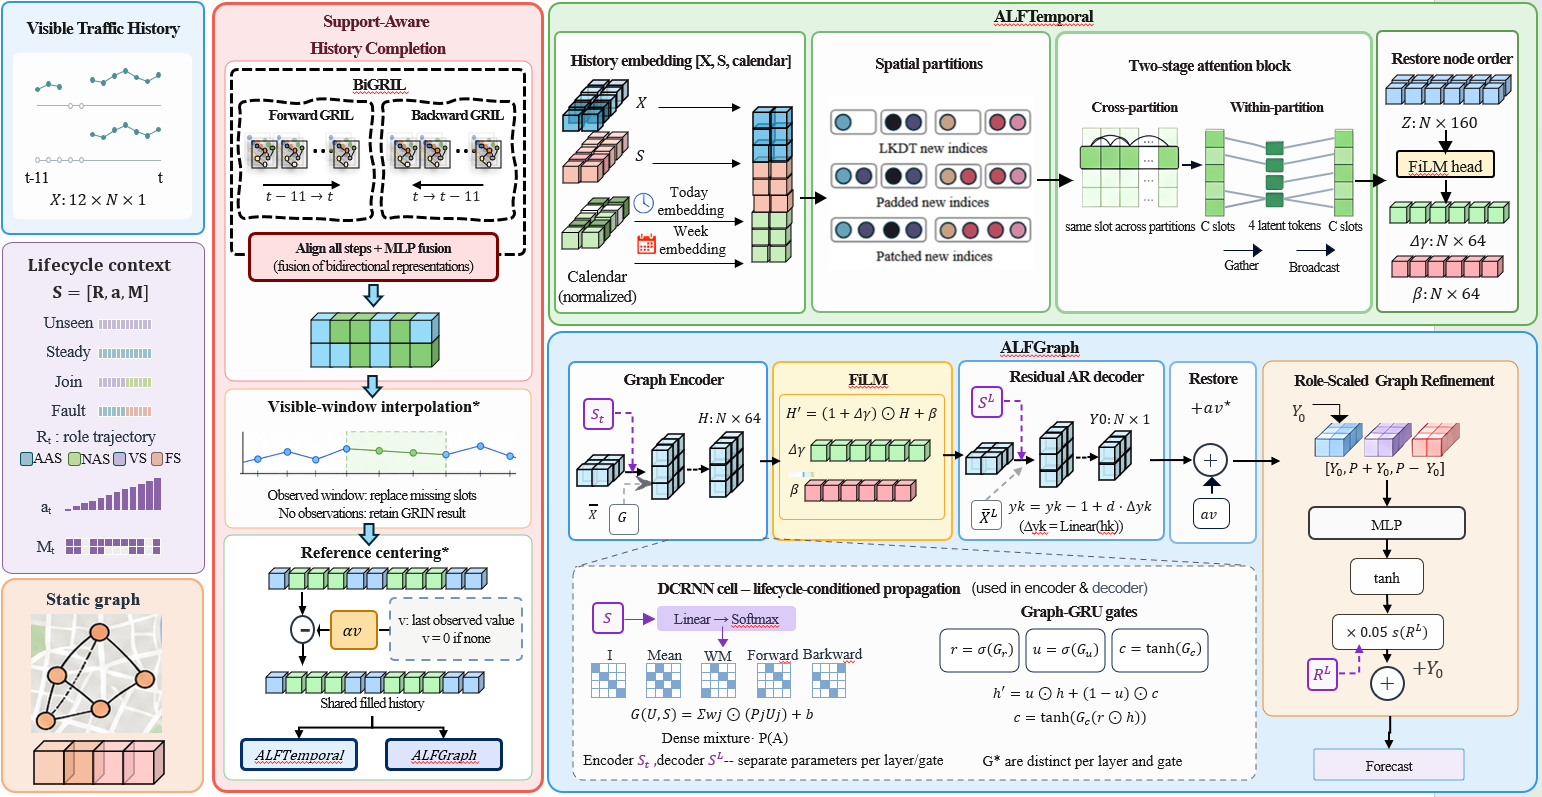
\includegraphics[width=\textwidth]{figures/alfnet.png}
\caption{\textbf{动态观测支持下的 ALFNet 架构。}共享的 GRIN/BiGRIL 模块对全部节点重建完整的12步历史，前向与后向递推对齐后合并；观测值保持不变，缺失位置被补全，并按数据集施加窗口插值（仅对至少有一个可见读数、$q>0$ 的节点）与参考中心化（$\bar{\mathbf{X}}=\mathbf{X}^{\mathrm{fill}}-\alpha\mathbf{v}$，$\mathbf{v}$ 为最后一次可见读数，无观测时为0），得到两个分支共享的历史 $\bar{\mathbf{X}}$。ALFTemporal 以步长为12的卷积将每个节点的窗口压缩为一个64维时间 patch，拼接日内时刻、星期与共享结构嵌入（160维），将节点组织为 $P=32$ 个各含 $C$ 个槽位的空间分区，经一个两阶段注意力块——同一槽位的跨分区注意力，以及经4个潜在 token 的分区内汇聚与回传——后恢复节点顺序。FiLM 参数头将所得 $\mathbf{Z}\in\mathbb{R}^{N\times160}$ 映射为 $(\Delta\boldsymbol{\gamma},\boldsymbol{\beta})$，在解码前一次性调制两层图编码器的末状态。ALFGraph 使用生命周期条件化的 DCRNN 单元，其各门以基于生命周期状态的 softmax 路由稠密组合五种传播支持；两层残差自回归解码器以 $\bar{\mathbf{X}}_L$ 为初值，并回送未经修正的逐步预测。加回 $\alpha\mathbf{v}$ 后，角色缩放图修正施加由末步角色 $\mathbf{R}_L$ 缩放的有界邻域残差，得到唯一的12步预测 $\hat{\mathbf{Y}}$。Unseen、Steady、Join 与 Fault 表示观测场景，由随时间变化的角色（AAS/NAS/VS/FS）、状态年龄与观测掩码实现。*数据集特定处理：METR-LA/PEMS-BAY/PEMS04/PEMS08 的 $C$=7/16/10/6，插值为关/关/开/开，解码残差倍率 $d$=0.3/0.3/1/1，$\alpha$=0/0/0/0.5。每层每个门各有独立路由；加权均值（WM）与前向扩散（Fwd）两种支持的传播形式相同但参数独立；每个注意力阶段均含残差、归一化与前馈层。图中省略批量维度，曲线与矩阵元素为示意。}
\label{fig:arch}
\end{figure}

ALFNet（Adaptive Lifecycle Forecasting Network）的“自适应”指计算随输入的观测支持而变化，推理时模型参数保持固定。如图\ref{fig:arch}所示，观测支持感知历史补全（Support-Aware History Completion，SAHC）首先为全部节点生成共享历史 $\bar{\mathbf{X}}$。随后两个分支读取同一份 $\bar{\mathbf{X}}$ 与 $\mathbf{S}$：ALFTemporal 从跨节点历史生成条件特征 $\mathbf{Z}$，经 FiLM 参数头调制 ALFGraph 的编码末状态；ALFGraph 以观测状态决定图传播的组合方式，完成编码与残差自回归解码。解码输出加回中心化参考值后，经角色缩放图修正得到唯一预测。两个分支共享输入张量与补全器，但不共享各自的主干参数；图\ref{fig:arch}中的并列表示依赖关系，计算上先得到时间分支的调制参数，再执行图分支。

各组成部分沿用了已有算子：图循环插补来自 GRIN~\citep{cini2022filling}，扩散卷积循环单元与门控循环单元（gated recurrent unit, GRU）分别来自 DCRNN 与 Cho 等人的工作~\citep{li2018diffusion,cho2014learning}，传播算子的专家组合参考 MoGERNN 与稀疏专家混合~\citep{zhou2025mogernn,shazeer2017outrageously,wang2023graph}，空间分区组织来自 PatchSTG~\citep{fang2025efficient}，两阶段注意力改编自 Crossformer~\citep{zhang2023crossformer}，特征调制采用 FiLM~\citep{perez2018film}。本文的方法贡献在于以观测支持组织这些计算，具体落实为三项设计选择，并分别由\ref{sec:4_4}节的消融检验：（i）图传播的组合只由逐步的观测状态决定，不读取信号值，使补全之后实测读数与补全读数仍可区分（w/o Adaptive Routing）；（ii）跨节点时间上下文只作为条件，在编码末状态注入一次，不形成独立预测（w/o Spatial Context、w/o ALFTemporal–FiLM）；（iii）状态年龄为接入与中断的进展提供显式条件（w/o State Age）。与 MoGERNN 中稀疏选择的图专家混合~\citep{zhou2025mogernn} 不同，ALFNet 把传播算子的专家组合放进循环单元的每个门，由生命周期上下文稠密路由。观测支持感知历史补全与角色缩放图修正是配合这三项选择的设计组件，正文没有对它们单独做消融。

\subsection{观测支持感知历史补全（SAHC）}\label{sec:3_3}

共享补全对全部 $N$ 个节点、完整的 $L$ 步历史只运行一次：
\begin{equation}\label{eq:2}
\mathbf{X}^{\mathrm{grin}}=\mathbf{M}\odot\mathbf{X}+(\mathbf{1}-\mathbf{M})\odot\mathbf{X}^{\mathrm{rec}},\qquad
\mathbf{X}^{\mathrm{rec}}=\mathrm{BiGRIL}\big(\mathbf{X}\odot\mathbf{M},\ \mathbf{M},\ [\mathbf{R},\mathbf{a}];\ \mathbf{A}\big).
\end{equation}

BiGRIL 沿时间正、反两个方向各运行一个图循环插补层~\citep{cini2022filling}：每一步先由上一隐藏状态给出初步估计，再经空间消息传递修正，以观测值替换可见位置后更新图循环状态；两个方向在每个历史位置上的表示与掩码经多层感知机（MLP）融合，得到重建 $\mathbf{X}^{\mathrm{rec}}$。角色与年龄作为外生输入进入两个方向的递推，掩码单独使用。补全器没有独立的重建损失，只通过下游预测损失训练；正文没有对共享补全单独做消融。

对流量数据，补全之后再施加两项固定的输入处理。其一是窗口内插值：
\begin{equation}\label{eq:3}
X^{\mathrm{fill}}_{t,n}=
\begin{cases}
\mathrm{Interp}(\mathbf{X}_{:,n},\mathbf{M}_{:,n})_t, & \text{插值开启},\ M_{t,n}=0,\ q_n>0,\\
X^{\mathrm{grin}}_{t,n}, & \text{其他情况},
\end{cases}
\end{equation}
其中 $\mathrm{Interp}$ 只使用当前窗口内的可见读数：两个可见读数之间线性插值，窗口两端之外取最近的可见值。没有可见读数（$q_n=0$）的节点保留 GRIN 由图消息传递得到的补全值。因此，插值与 GRIN 不是按 $q$ 互斥的两条支路：所有节点先经过 GRIN，插值只覆盖至少有一个可见读数的节点的缺失位置。其二是参考中心化：
\begin{equation}\label{eq:4}
\bar{\mathbf{X}}=\mathbf{X}^{\mathrm{fill}}-\alpha\,\mathbf{v},
\end{equation}
其中 $v_n$ 为窗口内最后一个可见的标准化读数，无可见读数时 $v_n=0$，并沿时间维广播；$\alpha$ 为固定的中心化强度，$\mathbf{S}$ 保持不变。中心化在输出端对应加回（\ref{sec:3_4}节）。速度数据不插值、不中心化，此时 $\bar{\mathbf{X}}=\mathbf{X}^{\mathrm{grin}}$。上述处理均不使用未来或被遮蔽的真值。保留观测值发生在中心化之前；中心化后，可见位置的数值也随之平移。两个分支读取同一份 $\bar{\mathbf{X}}$。

\subsection{观测条件化图预测（ALFGraph）}\label{sec:3_4}

\textbf{生命周期条件化图传播。} ALFGraph 以 DCRNN 的扩散卷积循环结构为基础~\citep{li2018diffusion}，将门控中的单一传播算子替换为五种传播支持的条件化组合。五种支持依次为恒等矩阵 $\mathbf{P}_1=\mathbf{I}$、二值邻接的行归一化 $\mathbf{P}_2$、加权邻接的行归一化 $\mathbf{P}_3$，以及 $\mathbf{A}$ 与 $\mathbf{A}^{\top}$ 的随机游走转移矩阵 $\mathbf{P}_4$、$\mathbf{P}_5$。在非负邻接上，$\mathbf{P}_3$ 与 $\mathbf{P}_4$ 的归一化形式相同，但二者具有独立的投影参数与路由权重。对第 $t$ 步，路由器只读取生命周期上下文：
\begin{equation}\label{eq:5}
\mathbf{w}_t=\mathrm{softmax}\big(\mathbf{S}_t\mathbf{W}_g\big)\in\mathbb{R}^{N\times5},
\end{equation}
softmax 沿专家维对每个节点分别计算。给定门控输入 $\mathbf{U}\in\mathbb{R}^{N\times F}$，条件化传播为
\begin{equation}\label{eq:6}
G(\mathbf{U},\mathbf{S}_t)=\sum_{j=1}^{5}\mathbf{w}_{t,j}\odot\big(\mathbf{P}_j\,\mathbf{U}\,\boldsymbol{\Theta}_j\big)+\mathbf{b},
\end{equation}
其中 $\mathbf{w}_{t,j}\in\mathbb{R}^{N}$ 沿特征维广播，$\boldsymbol{\Theta}_j\in\mathbb{R}^{F\times64}$ 为第 $j$ 个支持的投影。五个支持全部参与加权，不做 top-$k$ 截断，也不加入噪声。路由器读取观测状态而非信号值：经过共享补全后，一个新接入（NAS）节点与一个活跃（AAS）节点可能具有相似的输入数值，而二者的生命周期上下文仍然不同。

\textbf{图门控循环单元（GRU）。} 编码器第 $t$ 步的输入为 $\mathbf{x}_t=[\bar{\mathbf{X}}_t,\mathbf{S}_t]\in\mathbb{R}^{N\times7}$。每个门使用一个条件化传播模块：
\begin{equation}\label{eq:7}
\begin{aligned}
\mathbf{r}&=\sigma\big(G_r([\mathbf{x}_t,\mathbf{h}],\mathbf{S}_t)\big),\quad
\mathbf{u}=\sigma\big(G_u([\mathbf{x}_t,\mathbf{h}],\mathbf{S}_t)\big),\\
\mathbf{c}&=\tanh\big(G_c([\mathbf{x}_t,\mathbf{r}\odot\mathbf{h}],\mathbf{S}_t)\big),\quad
\mathbf{h}'=\mathbf{u}\odot\mathbf{h}+(1-\mathbf{u})\odot\mathbf{c},
\end{aligned}
\end{equation}
其中 $\sigma(\cdot)$ 为 sigmoid，隐藏宽度为64。编码器与解码器各有两层，每层的三个门各有独立的传播参数与路由器，共12个条件化传播模块；各模块的参数在递推步之间共享。编码器沿 $t=1,\dots,L$ 递推，得到两层的末状态 $\mathbf{H}^{\mathrm{enc}}=(\mathbf{h}^{(1)}_L,\mathbf{h}^{(2)}_L)$。由于角色与年龄逐步进入路由，Join 节点在接入前后、Fault 节点在中断前后会使用不同的传播组合。

\textbf{残差自回归解码与参考恢复。} 解码器以经 FiLM 调制的编码末状态为初始隐藏状态（\ref{sec:3_5}节），以共享历史的末步作为初值 $\mathbf{y}_0=\bar{\mathbf{X}}_L$；该初值来自补全与中心化后的历史，不一定是最后一次真实观测。对 $k=1,\dots,H$：
\begin{equation}\label{eq:8}
\mathbf{y}_k=\mathbf{y}_{k-1}+d\cdot\mathrm{Linear}\big(\mathbf{h}^{(2)}_k\big),
\end{equation}
其中 $\mathbf{h}^{(2)}_k$ 为解码器第二层在输入 $\mathbf{y}_{k-1}$ 下更新后的隐藏状态，$d$ 为固定的解码残差倍率。解码阶段没有未来的观测状态，路由统一使用末步上下文 $\mathbf{S}_L$，不对未来角色演变建模。每步回送的是未经修正的 $\mathbf{y}_k$。训练时采用受合法目标掩码约束的教师强制，其比例在前40轮线性衰减至零，评价时关闭。完成 $H$ 步解码后加回中心化参考值：
\begin{equation}\label{eq:9}
\tilde{\mathbf{Y}}=[\mathbf{y}_1,\dots,\mathbf{y}_H]+\alpha\,\mathbf{v}.
\end{equation}
这一步只恢复\ref{sec:3_3}节减去的参考值，不是标准化的逆变换；误差计算时再用训练时段的标准化统计量还原到原始单位。

\subsection{空间上下文时间条件分支（ALFTemporal）与 FiLM 调制}\label{sec:3_5}

\textbf{时间 patch 嵌入。} 对每个节点，ALFTemporal 读取 $[\bar{\mathbf{X}},\mathbf{S},\tau/288,\delta/7]\in\mathbb{R}^{L\times9}$，其中 $\tau=12\cdot\text{hour}+\lfloor\text{minute}/5\rfloor\in\{0,\dots,287\}$ 为日内时段（time of day, ToD），$\delta\in\{0,\dots,6\}$ 为星期（day of week, DoW）。卷积核长度与步长均为12的时间卷积将整个窗口压缩为一个64维向量 $\mathbf{e}_n$，因此每个节点只有一个时间 patch，窗口内读数的位置信息由卷积权重保留。随后拼接
\begin{equation}\label{eq:10}
\mathbf{z}^{0}_n=\big[\mathbf{e}_n\ \|\ \mathbf{E}^{\mathrm{tod}}_{\tau_L}\ \|\ \mathbf{E}^{\mathrm{dow}}_{\delta_L}\ \|\ \phi(\mathbf{g}_n)\big]\in\mathbb{R}^{160},
\end{equation}
其中 $\mathbf{E}^{\mathrm{tod}}$、$\mathbf{E}^{\mathrm{dow}}$ 为末步日内时段与星期的32维嵌入。结构嵌入 $\phi(\mathbf{g}_n)$ 由所有节点共享的多层感知机（MLP，7$\to$64$\to$32）作用于静态属性 $\mathbf{g}_n\in\mathbb{R}^7$ 得到：两维坐标、入度、出度、总加权度、对数总度与孤立标志；无坐标的数据集坐标置零。模型不使用逐节点可训练的身份嵌入，以免为保留节点引入可训练的身份参数。

\textbf{分区空间上下文编码。} 参照 PatchSTG 的空间分区组织~\citep{fang2025efficient}，节点被划分为 $P=32$ 个分区，每个分区含 $C$ 个槽位：速度数据依据已核验的地理坐标以 KD-tree 划分，流量数据依据图拓扑做考虑连通分量的广度优先搜索（BFS）划分。节点不足 $C$ 个的分区以邻接排序的真实节点补足，这些补足副本只提供上下文，不产生输出。分区后的特征经一个两阶段注意力块处理，该结构改编自 Crossformer~\citep{zhang2023crossformer}，单头，各阶段均含残差连接、层归一化与前馈层。第一阶段为\textbf{跨分区注意力}：对每个槽位索引 $c$，在 $P$ 个分区的同位 token $\{\mathbf{z}_{p,c}\}_{p=1}^{P}$ 之间做自注意力；在 Crossformer 中该阶段沿时间轴进行，这里改为沿分区轴。第二阶段为\textbf{分区内潜在汇聚与回传}：每个分区 $p$ 有4个可学习的潜在 token $\mathbf{Q}_p\in\mathbb{R}^{4\times160}$，
\begin{equation}\label{eq:11}
\mathbf{B}_p=\mathrm{Attn}\big(\mathbf{Q}_p,\mathbf{Z}_p,\mathbf{Z}_p\big),\qquad
\mathbf{Z}_p\leftarrow\mathrm{Attn}\big(\mathbf{Z}_p,\mathbf{B}_p,\mathbf{B}_p\big),
\end{equation}
其中 $\mathbf{Z}_p\in\mathbb{R}^{C\times160}$ 为分区内的槽位特征。潜在 token 先从 $C$ 个槽位汇聚信息，再回传给各槽位，分区内的交互因此经过4个 token 的瓶颈，而不是 $C\times C$ 的直接注意力。处理后按原始节点顺序取回，得到条件特征 $\mathbf{Z}\in\mathbb{R}^{N\times160}$。ALFTemporal 不产生独立的预测，只为图分支提供条件。

\textbf{FiLM 调制。} FiLM 参数头将 $\mathbf{Z}$ 映射为逐节点的缩放与平移参数，并调制两层编码末状态~\citep{perez2018film}：
\begin{equation}\label{eq:12}
(\Delta\boldsymbol{\gamma},\boldsymbol{\beta})=\mathrm{MLP}_{160\to32\to128}(\mathbf{Z}),\qquad
\mathbf{h}^{(l)}_{\mathrm{mod}}=(1+\Delta\boldsymbol{\gamma})\odot\mathbf{h}^{(l)}_L+\boldsymbol{\beta},\quad l=1,2,
\end{equation}
其中 $\Delta\boldsymbol{\gamma},\boldsymbol{\beta}\in\mathbb{R}^{N\times64}$。参数头的最后一层零初始化，训练开始时调制为恒等映射。同一组参数广播到两层，只在编码完成、解码开始之前作用一次，不在每个预测步重新生成。观测支持对 FiLM 参数的影响只经由 ALFTemporal 的输入，参数头与 $\mathbf{S}$ 之间没有直接连接。

\subsection{角色缩放图修正}\label{sec:3_6}

解码与参考恢复之后，输出端施加一个有界的邻域修正。令 $\mathbf{P}^{+}$、$\mathbf{P}^{-}$ 分别为 $\mathbf{A}+\mathbf{I}$ 及其转置的行归一化矩阵，
\begin{equation}\label{eq:13}
\mathbf{D}=\mathrm{Linear}_{32\to1}\Big(\mathrm{GELU}\big(\mathrm{Linear}_{3\to32}([\tilde{\mathbf{Y}},\ \mathbf{P}^{+}\tilde{\mathbf{Y}},\ \mathbf{P}^{-}\tilde{\mathbf{Y}}])\big)\Big),\qquad
\hat{\mathbf{Y}}=\tilde{\mathbf{Y}}+0.05\cdot s(\mathbf{R}_L)\odot\tanh(\mathbf{D}),
\end{equation}
其中拼接沿每个预测步、每个节点的特征维进行，$s(\cdot)$ 为按末步角色取值的固定倍率，AAS、NAS、VS、FS 依次为0、1、1、0.25。最后一层零初始化；由于 tanh 有界，修正量的绝对值在标准化单位下不超过0.05。末步角色为活跃（AAS）的节点自身不被修正，但仍作为邻居参与其他节点的修正。该模块只读取末步角色，不读取年龄与掩码，也没有独立的路由器；修正结果不回送解码器。正文没有对该模块单独做消融。

\subsection{训练目标}\label{sec:3_7}

令 $e=|\hat{y}-y|$ 为原始单位下的绝对误差，$\sigma_{\mathrm{data}}$ 为训练时段目标变量的标准差。逐元素损失为
\begin{equation}\label{eq:14}
\ell(e)=\frac{e}{\sigma_{\mathrm{data}}}\tanh(0.1\,e).
\end{equation}
该损失在小误差附近近似 $0.1e^2/\sigma_{\mathrm{data}}$，大误差时趋近标准化 MAE；权重项参与梯度计算。四个数据集取相同系数，但 $e$ 分别以各自的速度或流量单位计量，因此相同系数并不意味着跨量纲的同等加权。记 $\Omega$ 为一个批次内有效的目标元素，$\Omega_r$ 为其中末步角色为 $r$ 的节点所对应的元素，$\mathcal{R}_b$ 为该批次实际出现的角色集合，则
\begin{equation}\label{eq:15}
\mathcal{L}_{\mathrm{mean}}=\frac{1}{|\Omega|}\sum_{\Omega}\ell(e),\qquad
\mathcal{L}_{\mathrm{role}}=\frac{1}{|\mathcal{R}_b|}\sum_{r\in\mathcal{R}_b}\frac{1}{|\Omega_r|}\sum_{\Omega_r}\ell(e),\qquad
\mathcal{L}=0.9\,\mathcal{L}_{\mathrm{mean}}+0.1\,\mathcal{L}_{\mathrm{role}}+\mathcal{L}_{\mathrm{route}}.
\end{equation}
$\mathcal{L}_{\mathrm{role}}$ 使样本较少的角色在优化中获得与其他角色相同的权重。$\mathcal{L}_{\mathrm{route}}$ 为路由平衡项~\citep{shazeer2017outrageously,wang2023graph}：每个条件化传播模块在每次调用时计算 $0.01\,[\mathrm{CV}^2(\text{importance})+\mathrm{CV}^2(\text{load})]$，其中 importance 为批次内各专家路由权重之和，$\mathrm{CV}^2$ 为平方变异系数；先在递推调用间取平均，再对12个模块取平均。由于五个支持全部参与加权，load 项恒为零，起作用的是 importance 项。训练目标不含独立的重建损失或额外预测头。该目标是对现有训练方式的描述，不作为独立的方法贡献。

\subsection{数据集特定设置}\label{sec:3_8}

四个数据集共享\ref{sec:3_3}–\ref{sec:3_7}节的同一可学习结构，参数量均为1,037,529。数据集之间的差异仅在于训练前固定的设置：分区容量 $C$（METR-LA、PEMS-BAY、PEMS04、PEMS08 依次为7、16、10、6），窗口插值（速度数据关闭、流量数据开启），解码残差倍率 $d$（0.3、0.3、1、1）与中心化强度 $\alpha$（0、0、0、0.5）。这些设置不可学习，也不在推理时由路由选择；完整取值与训练超参数见\ref{sec:4_1}节。它们按变量类型确定：速度数据不插值、解码残差倍率取0.3，流量数据采用窗口插值与倍率1，中心化只在 PEMS08 上使用。这些取值是在本文数据上经验选择的结果（选择过程见\ref{sec:4_1}节），没有可直接迁移到新路网的选择规则；在新路网上需要用验证集重新确定。
